\documentclass[a4paper,11pt]{article}

\usepackage[utf8]{inputenc}
\usepackage[T1]{fontenc}
\usepackage[english]{babel}

\usepackage{graphicx} % Inclusion d'images
\usepackage{amsfonts} % Symboles maths
\usepackage{amsmath} % Aligner les équations
\usepackage{fullpage} % Marges
\usepackage{xspace} % Espace après macros
\usepackage{float} % Positionnement des images
\usepackage{subcaption} % sous-legendes
\usepackage{units}

\title{Robotics project}
\author{BLÉRON Alexandre \& MEYRON Jocelyn}
\date{December, 14th 2014}

\begin{document}

\maketitle

\section{Detection using stereo vision}
\subsection{Segmentation in Cartesian Space}
We first implemented the road detection by converting back the disparity values into 3D points and filtering all points below a certain threshold.\\
Figure \ref{threshold-comparison} compares the filtered disparity maps for image pair 250 for different threshold values.

\begin{figure}[H]
\centering
\begin{minipage}{0.32\linewidth}
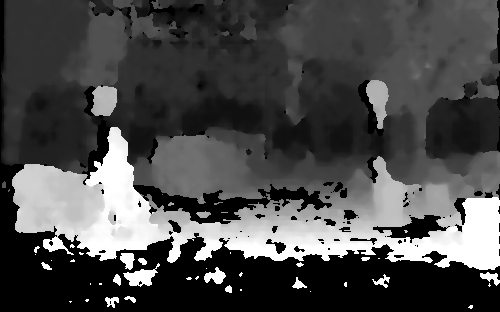
\includegraphics[scale=0.25]{pic/cartesian-00m.png}
\subcaption{$ Z < \unit[0.0]{m} $}
\label{threshold-comparison:a}
\end{minipage}
\begin{minipage}{0.32\linewidth}
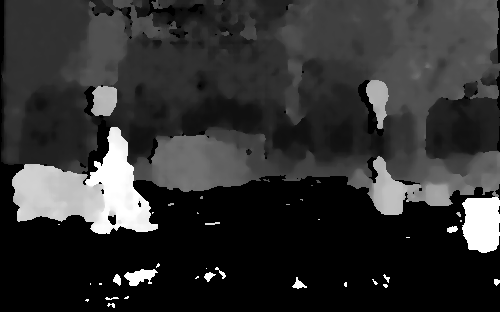
\includegraphics[scale=0.25]{pic/cartesian-02m.png}
\subcaption{$ Z < \unit[0.2]{m} $}
\label{threshold-comparison:b}
\end{minipage}
\begin{minipage}{0.32\linewidth}
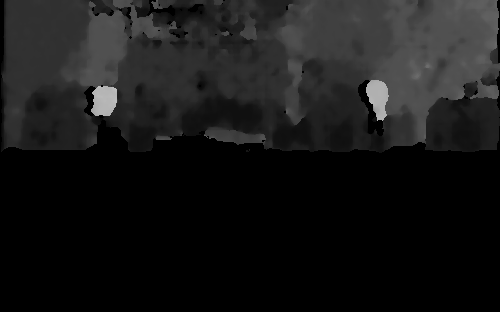
\includegraphics[scale=0.25]{pic/cartesian-20m.png}
\subcaption{$ Z < \unit[2.0]{m} $}
\label{threshold-comparison:c}
\end{minipage}
\caption{Comparison of different threshold values for road/obstacles segmentation}
\label{threshold-comparison}
\end{figure}

In figure \ref{threshold-comparison:a}, we can see that some pixels belonging to the road are not filtered. Figure \ref{threshold-comparison:b} shows reasonable results for $ Z < \unit[0.2]{m} $. As expected, figure \ref{threshold-comparison:c}, with threshold $ Z < \unit[2.0]{m} $ fails to detect low obstacles (such as the pedestrian).\\
We can also filter pixels above a certain height. Figure \ref{threshold-height} shows the same disparity map as \ref{threshold-comparison:b} with all pixels above \unit[2.5]{m} removed.

\begin{figure}[H]
\centering
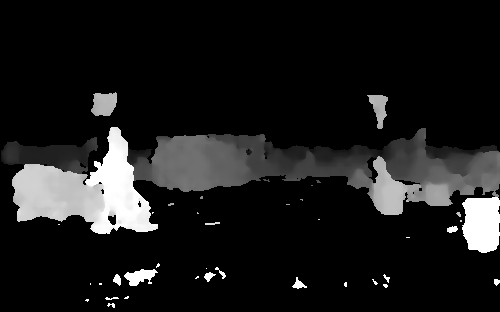
\includegraphics[scale=0.5]{pic/cartesian-02-25m.png}
\caption{Disparity map with all pixels outside $\left[\unit[0.2]{m}; \unit[2.0]{m} \right]$ removed.}
\label{threshold-height}
\end{figure}

This way, only the relevant obstacles are kept in the filtered image.

% Other thresholds

\subsection{Segmentation in Disparity Space}
Road/obstacle segmentation can also be done in disparity space, using the \textit{v-disparity} image (figure \ref{v-disparity}).

\begin{figure}[H]
\centering
\begin{minipage}{0.32\linewidth}
\centering
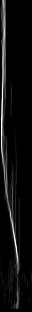
\includegraphics[scale=0.5]{pic/v-disparity.png}
\subcaption{Raw v-disparity map}
\label{v-disparity:a}
\end{minipage}
\begin{minipage}{0.32\linewidth}
\centering

\includegraphics[scale=0.5]{pic/v-disparity-threshold.png}
\subcaption{Denoised v-disparity map}
\label{v-disparity:b}
\end{minipage}
\caption{Calculated v-disparity map for image pair 250.}
\label{v-disparity}
\end{figure}

Figure \ref{v-disparity:b} shows the v-disparity map with values below 60 removed (set to zero). From this image, we can extract a line that represents the road surface.

\begin{figure}[H]
\centering

\includegraphics[scale=0.5]{pic/v-disparity-labeled.png}
\caption{Manually annotated v-disparity map. The measured line parameters are : position of the horizon line $ h_0 = 159 $, slope $ p_0 = -5.6 $ }
\label{ransac-line}
\end{figure}

Using the line parameters, we can estimate the height $Z_0$ and pitch angle $\theta$ of the camera:
\begin{align*}
\theta &= -atan(\frac{v_0-h_0}{\alpha_v}) \approx 0 \\
Z_0 &= -b\cdot\cos(\theta)\cdot p_0 \approx \unit[1.23]{m}
\end{align*} 

% h_0 and p_0 => \theta and Z_0
% Compare with cartesian space

We can filter out all the pixels that are located below the line in v-disparity space (for each entry $(u, v, d)$ in the disparity map, we get its location in v-disparity space with $(v, d)$). Figure \ref{v-disparity-comparison} shows a comparison between this method and cartesian segmentation.

\begin{figure}[H]
\centering
\begin{minipage}{0.45\linewidth}
\centering
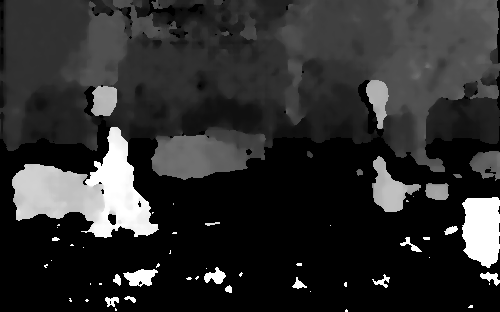
\includegraphics[scale=0.3]{pic/v-disparity-segmentation.png}
\subcaption{Segmentation using the v-disparity image}
\label{v-disparity-comparison:a}
\end{minipage}
\begin{minipage}{0.45\linewidth}
\centering
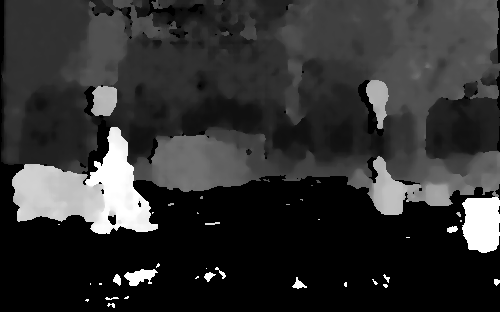
\includegraphics[scale=0.3]{pic/cartesian-02m.png}
\subcaption{Segmentation in cartesian space}
\label{v-disparity-comparison:b}
\end{minipage}
\caption{Comparison of disparity space segmentation and cartesian space segmentation.}
\label{v-disparity-comparison}
\end{figure}

The v-disparity method correctly isolates the road from the potential obstacles. It seems to reject more pixels than the cartesian method (the horizon line is higher), but this can be corrected by adjusting the rejection margin.  

\subsection{Clustering}
Before detecting potential obstacle in the image, we filter it using a morphological erosion followed by a dilatation (figure \ref{morpho-filter}).

\begin{figure}[H]
\centering
\begin{minipage}{0.45\linewidth}
\centering
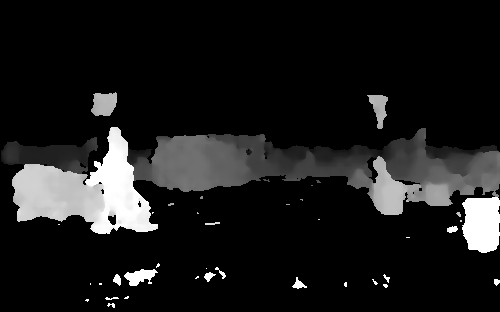
\includegraphics[scale=0.3]{pic/cartesian-02-25m.png}
\subcaption{Before filtering}
\label{morpho-filter:a}
\end{minipage}
\begin{minipage}{0.45\linewidth}
\centering
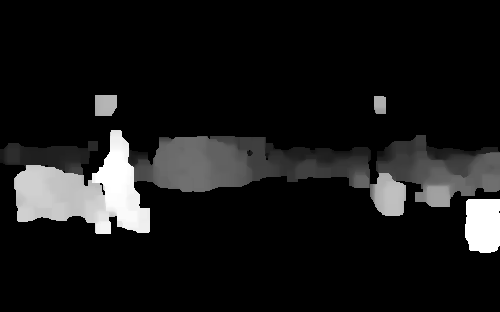
\includegraphics[scale=0.3]{pic/erode-dilate.png}
\subcaption{After filtering (kernel size = 10)}
\label{morpho-filter:b}
\end{minipage}
\caption{Pre-filtering of the segmented image. The small connected regions are removed.}
\label{morpho-filter}
\end{figure}

\newpage
\section{Tracking from laser scanner data}
Our state is composed of 4 parameters: the mean position and the velocity of
the region of interest. The observed measurement is the mean position (2
parameters).

The implementation is relatively straightforward: on the first frame, we know
the ROI so we can compute an initial position. We initialize our state with this
measurement. Then, for each frame, we compute the predicted value, we recenter
the ROI on this position. We finally correct the prediction by computing the
observed position (the mean position of the lidar impacts in the region of
interest).

Here are some screenshots for the tracking with a Kalman Filter. The blue cross
represents the observed position and the green cross the predicted one ($
\lambda $ is the variance of the noise during the measurement).

\begin{figure}[H]
    \centering
    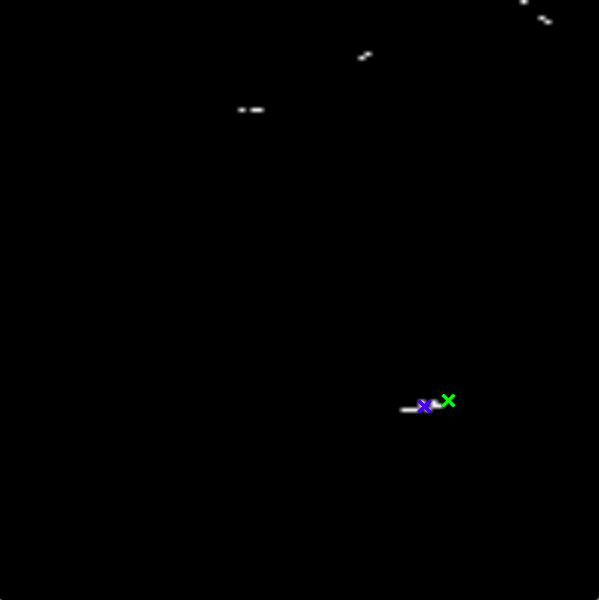
\includegraphics[scale=0.3]{pic/tracking1.png}
    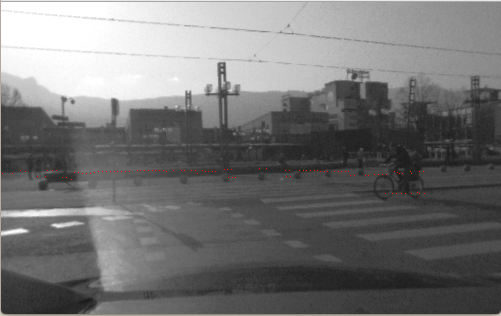
\includegraphics[scale=0.4]{pic/tracking1-left.png} \\
    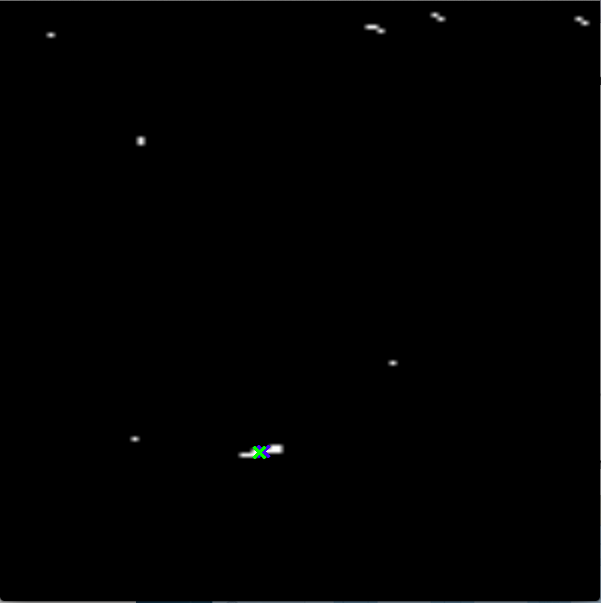
\includegraphics[scale=0.3]{pic/tracking2.png}
    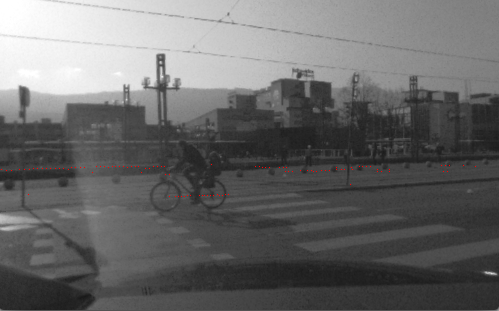
\includegraphics[scale=0.4]{pic/tracking2-left.png} \\
    \caption{Parameters: $ dt = 0.5 $ and $ \lambda = 1 $}
\end{figure}

The choice of the noise parameters is relatively important since if we choose,
for the covariance matrix of the noise, a diagonal with "high " values (50
for example), then the system is not able to track the ROI anymore. More precisely,
the higher the covariance matrix is, the more difficult it is for the system to
track the bicycle: at the beginning, the prediction is very far away from the
observed one and the time for the system to be closer the target precise
increases with the value of the covariance matrix.

Using the predicted state, we can estimate the speed of the bicycle. Using
\texttt{R}, we obtain the following graph. We filtered the last 5 frames because
the bicycle was not present in the scene anymore.

\begin{figure}[H]
    \centering
    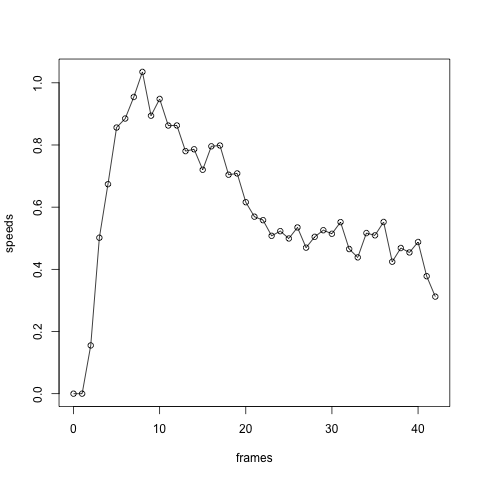
\includegraphics[scale=0.5]{pic/speed_estimation.png}
\end{figure}

The average estimated velocity is $ 0.588~m / s $ with a standard deviation of $ 0.232 $.

% Noise parameters influence?
% Estimate velocity of the target

\end{document}

